\documentclass[10pt]{article}
\usepackage{graphicx}
\usepackage{amssymb}
\usepackage[fleqn]{amsmath}
\usepackage{nccmath}
\usepackage{cases}
\usepackage{hyperref}
\usepackage{multicol}
\usepackage{tikz}
\usepackage{pgfplots}
\usepackage{enumitem}
\pgfplotsset{compat=1.18}
\usepackage{float}
\usepackage{pdfpages}
\DeclareMathOperator*{\lcm}{lcm}

\title{\bf Math 116: Problem Set 8}
\author{\bf Owen Jones}
\begin{document}
\maketitle
\begin{enumerate}[label= \arabic*.]
    \item Suppose plaintext $P=L_0R_0$ encrypts to ciphertext $C$. 
    Recall the structure of a Feistel cipher:
    \begin{align*}
        &L_i=R_{i-1}\quad R_i=L_{i-1}\oplus f(R_{i-1},K_i)
    \end{align*}
    Consider plaintext $\overline{P}=\overline{L_0R_0}$. 
    It suffices to show that after each round $i$, the output resulting from initial plaintext $\overline{P}$ and key $\overline{K_i}$ is the complement of the output resulting from initial plaintext $P$ and key $K_i$.
    \begin{align*}
        &\overline{R_0}\oplus\overline{K_1}=R_0\oplus 11111\ldots\oplus K_1\oplus 11111\ldots=R_0\oplus K_1\\
        &\Rightarrow f(\overline{R_0},\overline{K_1})=S(\overline{R_0}\oplus\overline{K_1})=S(R_0\oplus K_1)=f(R_{0},K_1)\text{ (inputs are the same)}\\
        &L_1'=\overline{R_0}=\overline{L_1}\quad R_1'=\overline{L_0}\oplus f(\overline{R_0},\overline{K_1})=\overline{L_0}\oplus f(R_{0},K_1)=\overline{R_1}\\
        &\Rightarrow L_1'R_1'=\overline{L_1}\overline{R_1}
    \end{align*}
    Suppose after i rounds $L_i'R_i'=\overline{L_i}\overline{R_i}$.
    \begin{align*}
        &L_{i+1}'=\overline{R_i}=\overline{L_{i+1}}=\quad R_{i+1}'=\overline{L_i}\oplus f(\overline{R_i},\overline{K_{i+1}})=\overline{L_i}\oplus f(R_{i},K_{i+1})=\overline{R_{i+1}}\\
        &\Rightarrow L_{i+1}'R_{i+1}'=\overline{L_{i+1}}\overline{R_{i+1}}
    \end{align*}
    Thus, by induction, the output resulting from initial plaintext $\overline{P}$ and key $\overline{K_i}$ is the complement of the output resulting from initial plaintext $P$ and key $K_i$ for all $i$.
    Hence, $\overline{P}$ encrypts to ciphertext $\overline{C}$.
    \item \begin{enumerate}
        \item Suppose $x_1\oplus x_2=x_3\oplus x_4$. Because XOR is linear
        \begin{align*}
            &f(x_1)\oplus f(x_2)=\alpha x_1+\beta\oplus \alpha x_2+\beta=\alpha(x_1\oplus x_2)+\beta\oplus \beta\\
            &=\alpha(x_3\oplus x_4)+\beta\oplus \beta=\alpha x_3+\beta\oplus \alpha x_4+\beta=f(x_3)\oplus f(x_4)
        \end{align*}, so $f$ has the equal difference property.
        \item Suppose $x_1\oplus x_2=x_3\oplus x_4$.
        \begin{itemize}
            \item [Shiftrow] Consider row $2$ of the ShiftRow matrix for input $x_k$ $c_2^{(k)}=\begin{bmatrix}
                c_{1,0} & c_{1,1} & c_{1,2} & c_{1,3}
            \end{bmatrix}=\begin{bmatrix}
                b_{1,1} & b_{1,2} & b_{1,3} & b_{1,0}
            \end{bmatrix}$. Observe $c_2^{(1)}\oplus c_2^{(2)}=c_2^{(3)}\oplus c_2^{(4)}$ because $b_{i,j}^{(1)}\oplus b_{i,j}^{(2)}=b_{i,j}^{(3)}\oplus b_{i,j}^{(4)}$ will hold for each byte in the $4\times 4$ matrix.
            Similarly, this will hold for any other row, so the output bit-strings $c^{(1)}\oplus c^{(2)}=c^{(3)}\oplus c^{(4)}$ will have this property. 
            \item [Mixcolumn] In part (a) we showed that an affine function has the equal difference property. For any byte in the output matrix, we have $d_{i,j}^{(k)}=\alpha_{i,j} c_{i,j}^{(k)}$ for some $alpha_{i,j}\in\mathbb{F}_{2^8}$. Thus, $d_{i,j}^{(1)}\oplus d_{i,j}^{(2)}=d_{i,j}^{(3)}\oplus d_{i,j}^{(4)}$ for every byte, so the output bit-strings $d^{(1)}\oplus d^{(2)}=d^{(3)}\oplus d^{(4)}$ will have this property.
            \item [RoundKey] $k_{i,j}\oplus d_{i,j}^{(1)}\oplus k_{i,j}\oplus d_{i,j}^{(2)}=d_{i,j}^{(1)}\oplus d_{i,j}^{(2)}=d_{i,j}^{(3)}\oplus d_{i,j}^{(4)}=k_{i,j}\oplus d_{i,j}^{(3)}\oplus k_{i,j}\oplus d_{i,j}^{(4)}$ for each byte in the $4\times 4$ matrix because $k_{i,j}\oplus k_{i,j}=00000\ldots$ and XOR is commutative.
            It follows this must also hold for the output bit-string.
        \end{itemize}
    \end{enumerate}
    \item \begin{enumerate}
        \item In $2b$ we showed that each of ShiftRow, MixColumn, and RoundKey have the equal difference property, so it's pretty trivial that their composition would have the equal difference property. 
        $x_1\oplus x_2=x_3\oplus x_4\Rightarrow f(x_1)\oplus f(x_2)=f(x_3)\oplus f(x_4)\Rightarrow g(f(x_1))\oplus g(f(x_2))=g(f(x_3))\oplus g(f(x_4))$ if both $f$ and $g$ have the equal difference property.
        \item In $2b$ we showed $k_{i,j}\oplus d_{i,j}^{(1)}\oplus k_{i,j}\oplus d_{i,j}^{(2)}=d_{i,j}^{(1)}\oplus d_{i,j}^{(2)}$ for each byte in the $4\times 4$ matrix.  
        Thus, $E(x_1)\oplus E(x_2)$ is only dependent on the ShiftRow and MixColumn steps.
        \item We can exploit the fact that $E(x_1)\oplus E(x_2)$ is independent of the key. We can apply InvMixColumn and InvShiftRow to $E(x_1)\oplus E(x_2)$ to obtain $x_1\oplus x_2$. This is also guaranteed by the equal difference property. We know $x_1$, so $x_1\oplus x_1\oplus x_2=x_2$.
    \end{enumerate}
    \item We have $x_1\oplus x_2=x_3\oplus x_4$. By $2a$, we would have $BS(x_1)\oplus BS(x_2)=BS(x_3)\oplus BS(x_4)$ if the ByteSub transformation was an affine map. However, we have a counterexample where that is not the case, so ByteSub transformation cannot be an affine map.
    \item $P_{j+1}=D_K(C_{j+1})\oplus C_{j}$ and $P_j=D_K(C_{j})\oplus C_{j-1}$ will be decrypted incorrectly because they are all of the blocks that depend on $C_j$.
    \item Suppose $x$ and $y$ are two messages such that $x\equiv y\pmod{p-1}$. Then $h(x)=h(y)$, so we will have multiple messages with the same hash value. Moreover, if it's not computationally difficult to find $2$ messages with the same hash value. 
    \item \begin{enumerate}
        \item $a_0=1$
        \item $x\equiv 5\pmod{8}$
        \item $b_0=1$ $b_1=2$ $x\equiv 7\pmod{9}$
        \item $x\equiv 7\pmod{13}$
        \item $x=709$ by CRT
    \end{enumerate}
    \item $x\equiv 2\pmod{4}$, $x\equiv 14\pmod{27}$ $x\equiv 7\pmod{11}$ By CRT $x\equiv 986\pmod{1188}$
\end{enumerate}
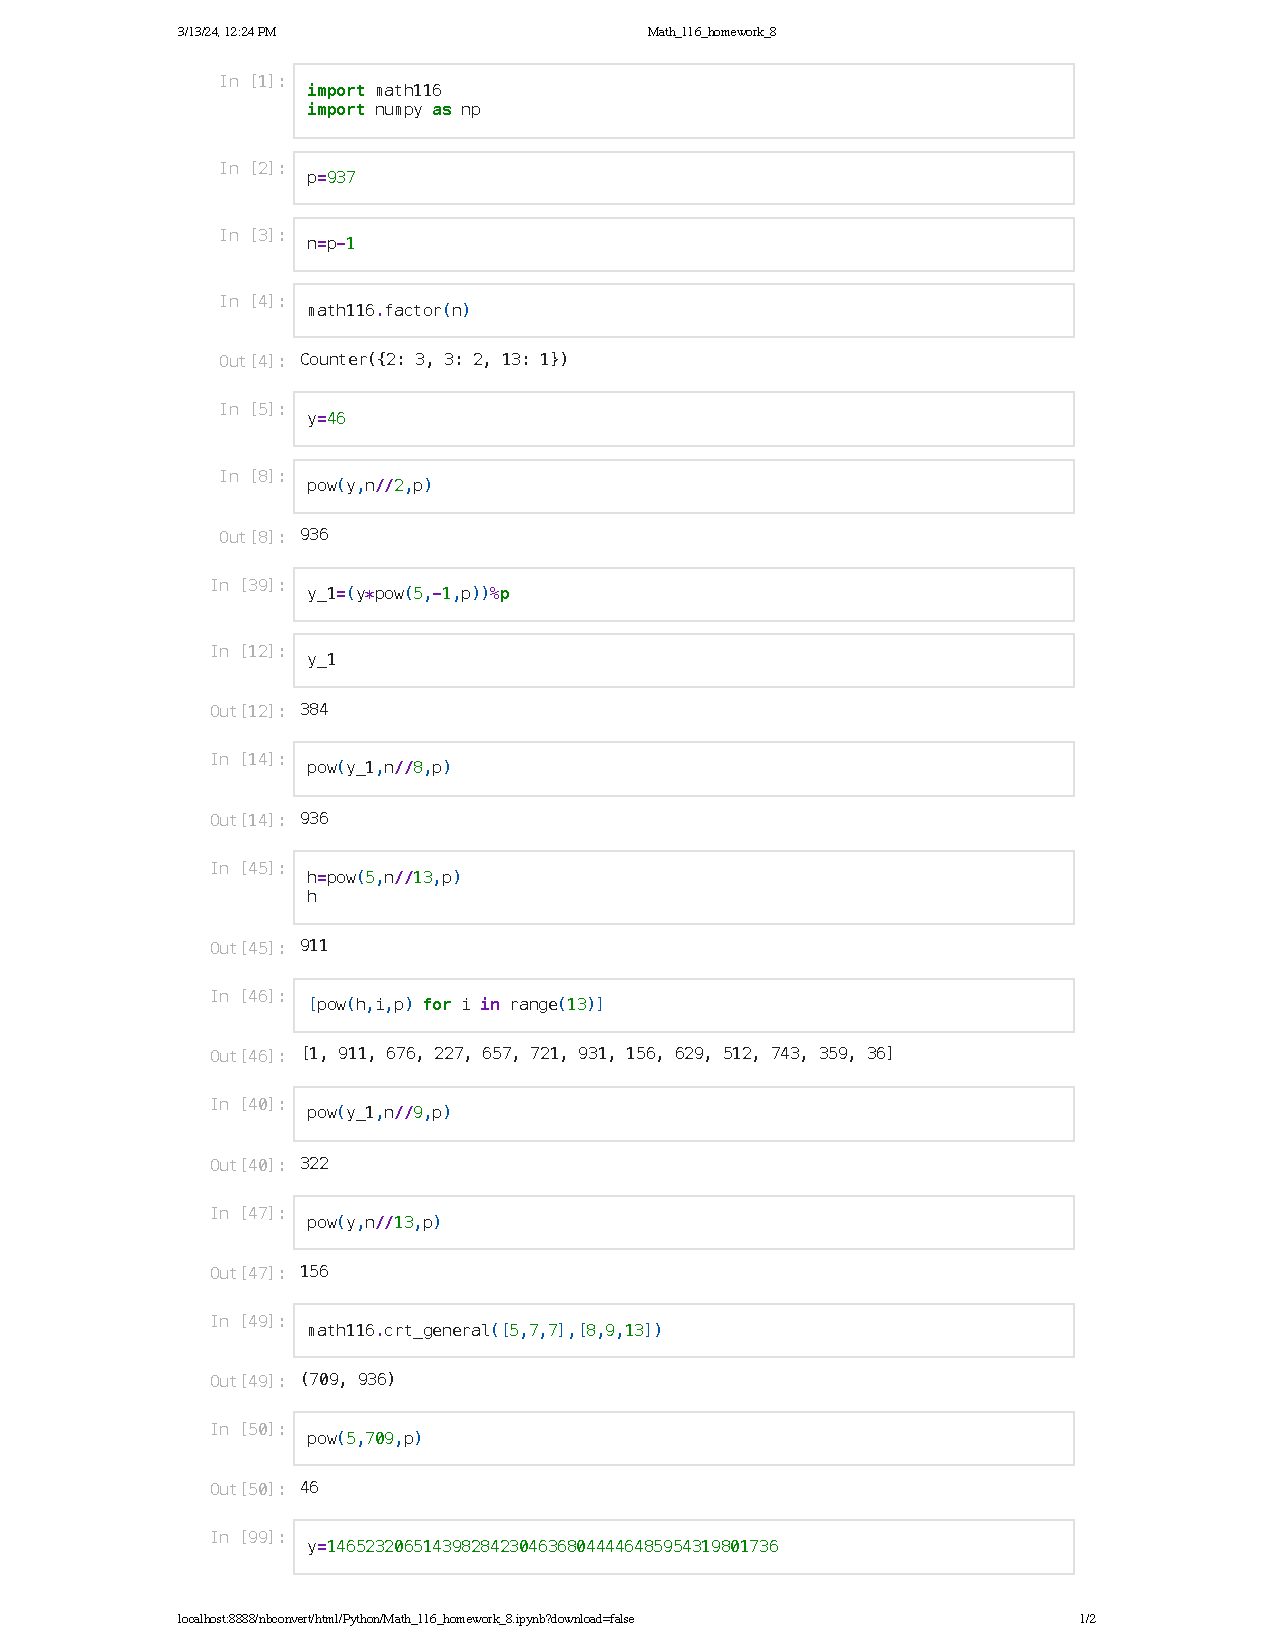
\includepdf[pages=-]{Math_116_homework_8_python.pdf}
\end{document}